% Training dynamics: AC plateau vs TR overfit
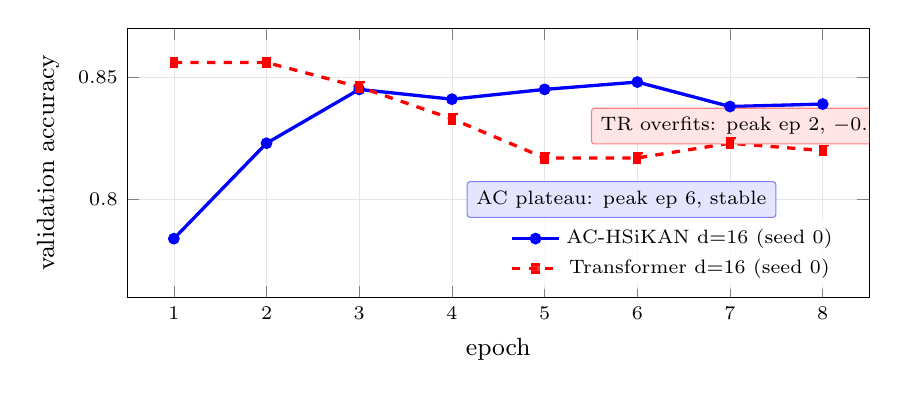
\begin{tikzpicture}
\begin{axis}[
  width=11cm, height=5cm,
  xlabel={epoch},
  ylabel={validation accuracy},
  xlabel style={font=\small},
  ylabel style={font=\small},
  tick label style={font=\scriptsize},
  xmin=0.5, xmax=8.5,
  ymin=0.76, ymax=0.87,
  xtick={1,2,3,4,5,6,7,8},
  grid=both,
  major grid style={lightgray!40, very thin},
  minor grid style={lightgray!20, very thin},
  legend pos=south east,
  legend style={font=\scriptsize, draw=none, fill=white, fill opacity=0.8, text opacity=1},
]

% AC-HSiKAN (seed 0 from /tmp/imdb_full_5seed_today.json)
\addplot[blue, very thick, mark=*, mark size=1.5pt] coordinates {
  (1, 0.784) (2, 0.823) (3, 0.845) (4, 0.841)
  (5, 0.845) (6, 0.848) (7, 0.838) (8, 0.839)
};
\addlegendentry{AC-HSiKAN d=16 (seed 0)}

% Transformer (seed 0 same file)
\addplot[red, very thick, dashed, mark=square*, mark size=1.5pt] coordinates {
  (1, 0.856) (2, 0.856) (3, 0.846) (4, 0.833)
  (5, 0.817) (6, 0.817) (7, 0.823) (8, 0.820)
};
\addlegendentry{Transformer d=16 (seed 0)}

% Annotate dynamics
\node[font=\scriptsize, anchor=west, fill=red!10, draw=red!50, rounded corners=1pt]
  at (axis cs:5.5, 0.83) {TR overfits: peak ep 2, $-0.04$ by ep 8};
\node[font=\scriptsize, anchor=east, fill=blue!10, draw=blue!50, rounded corners=1pt]
  at (axis cs:7.5, 0.80) {AC plateau: peak ep 6, stable};

\end{axis}
\end{tikzpicture}
